%\documentclass[preprint2,numberedappendix,tighten,twocolappendix]{aastex6}  % USE THIS TO MAKE BIB, THEN FORMAT USING EMULATEAPJ
\documentclass[twocolumn,apj,numberedappendix]{emulateapj}
\shorttitle{Adding Sensitivity to 21\,cm Inteferometric Probes of Reionization}
\shortauthors{Zhang, Liu \&Parsons}
\usepackage{float}
\usepackage{amsmath}
\usepackage{graphicx}
\usepackage[figuresright]{rotating}
%\usepackage{rotating}
\usepackage{natbib}
%\usepackage{pdflscape}
%\usepackage{lscape}
\usepackage{ctable}
\citestyle{aa}
\renewcommand\[{\begin{equation}}
\renewcommand\]{\end{equation}}
\graphicspath{{../figures/}}

\begin{document}

\title{A Generalized Visbility to Power-Spectrum Framework for 21\,cm Inteferometric Probes of Reionizations}

%\maketitle
\author{
Yunfan Gerry Zhang \altaffilmark{1},
Adrian C. Liu \altaffilmark{1, 2},
Aaron R. Parsons\altaffilmark{1, 2}
}

\altaffiltext{1}{Astronomy Dept., U. California, Berkeley, CA}
\altaffiltext{2}{Radio Astronomy Lab., U. California, Berkeley, CA}

\begin{abstract}
The observational effort to measure the cosmological 21\,cm power spectrum with radio interferometers requires high sensitivity. Current visibility-based power spectrum pipelines, though shown to ease control of systematics, lack the ability to include partial redundancy. We introduce a method to include partial redundancy in such power spectrum pipelines of drift-scan arrays. Our method efficiently finds pairs of baselines to cross-multiply, and quantifies the sensitivity contributions of given baselines. 
Using the 128-element configurations and beams of the Precision Array for Probing the Epoch of Reionization (PAPER-128), as well as 4 planned versions of the Hydrogen Epoch of Reionization Array (HERA), we illustrate how our method applies to different arrays and predict the sensitivity improvements of including each baseline pairs. We show that inclusion of partially redundant baselines 
would account for $20\%$ to $60\%$ of the sensitivity of PAPER-128 and different configurations of HERA. 
\end{abstract}

\section{Introduction}

The epoch of reionization represents the last key
stage of our Universe's early evolution. Study of this event stands at
the intersection of cosmology and astrophysics. Understanding this
event not only serves as a scientific goal
of its own, but also as a gateway to crucial information
regarding fundamental physics of inflation, neutrino mass and phenomenology
of the first stars and galaxies (e.g. \citealt{LiuOpticalDepth, Liu2016b, Mao2008, DEw21cm, Bull2015, Oyama20131186}). 

In the past, observational studies of reionization, including Gunn-Peterson measurements of quasi-stellar objects \citep{Fan2006} and cosmic microwave background (CMB) measurements of temperature and anisotropy \citep{Planck2016}, Kinetic Sunyaev-Zeldo'vich effect \citep{kszpatchy} and and Lyman alpha emitter clustering \citep{mcquinnLyA} have given us indications of the rough time-frame of reionization, but only limited constrains on the finer spatial and temporal variations. A surge of recent radio-astronomical experiments of reionization focus on measurement of the ``spin-flip'' transition of neutral
hydrogen of characteristic wavelength 21\,cm \citep{Furlanetto2006181,PritchardLoeb}.
In complement to the aforementioned probes, the 21\,cm brightness temperature distribution is a direct tracer of neutral hydrogen through the epoch of reionization, and thus tomography of the 21\,cm line is a direct measurement of the full temporal and spatial variations of this event. 
Before possible realization of full scale 21\,cm tomography, many current radio interferometric efforts
prioritize measuring the spatial power spectrum of 21\,cm brightness temperature fluctuations.
Current-generation instruments include the Precision Array for Probing
the Epoch of Reionization (PAPER) \citep{Ali2015,paper32}, Murchison
Widefield Array (MWA) \citep{Bowman2013, Tingay2013}, Low Frequency Array (LOFAR) \citep{LOFAR}. Next-generation instruments include the Hydrogen Epoch of Reionization
Array (HERA) (e.g. \citealt{HERA,HERAconfiguration,HERABEAM1,HERADISH2})  under construction, 
and the Square Kilometer Array Low (SKA-low) (e.g. \citealt{SKA1}), which is currently in planning. 

The highly redshifted 21\,cm signal is faint and diffuse, in contrast to the localized bright sources that have been of interest in many traditional applications of radio astronomy.  Current experiments are sensitivity-starved, with the sensitivity requirement further increased considering the foreground contaminations 5 orders of magnitude brighter than the cosmological signal of interest. Thus modern low-frequency radio interferometers aimed at measuring the 21\,cm signal bears designs different from traditional instruments. Many specially designed arrays, such as PAPER and HERA, feature multiple copies of the same baselines to repeatedly measure the same Fourier signal to increase sensitivity. To satisfy the sensitivity need, modern arrays are large. Ranging upwards from 100 elements, these arrays are typically of the drift-scan type to limit cost.

Analysis pipelines for the 21\,cm power spectrum typically fall into two categories. In the first, more traditional technique, images are formed in Fourier domain through rotation synthesis, followed by a foreground mitigation step to construct a power spectrum. An alternative technique works directly with visibilities from baselines and cross multiplies them to form the power spectrum. Tracking closely the instrumental output of visibilities, this technique allows one to deal with systematics such as Radio-Frequency-Interference(RFI) and instrumental cross-talks in a more native context, and thus tend to provide good limits on the power spectrum. An example of the visibility-based pipeline was presented in \cite{Ali2015}, which provides the newest upper limit to the power spectrum
measurements with the 64-element version of PAPER (henceforth as PAPER-64). However, one disadvantage of existing visibility-based pipelines is the lack of use of partial redundancy. Baselines of different length and orientation still contain partially redundant information. While an imaging based power-spectrum pipeline naturally includes all redundancy information, visibility-based pipelines until now only cross multiply fully redundant baselines, in other words baselines of the same length and orientation.

The use of partially redundant baselines is in principle not a fundamental limitation of visibility-based pipelines. In fact, most instrumental reports to date do include partial redundancy. Recently, \cite{wterm} proposed a visibility-based approach to extract power spectrum from partially redundant baselines in tracking measurements. Arrays capable of tracking include MWA and LOFAR. Our work parallels this effort by focusing on drift-scan arrays that do not have tracking capabilities, such as PAPER, HERA and potentially SKA.
The Earth's rotation causes the baselines in a drift-scan array to pick up different modes of the sky with time. Rotation-synthesis makes use of the rotation-induced $uv$ coverage map to form image. In a visibility based pipeline, we can extract the same rotation-induced redundancy. In this point of view, baselines that are slightly different in length and orientation
``rotate into'' each other at a time delay. We can thus cross-multiply time-shifted visibilities, with the proper weighting, to form power spectra.  Due to the large number of elements of modern arrays (upward of 100), the task of cross-multiplying every baseline against every other, scaling as number of array elements to the fourth power, can be computationally formidable, and many pairs of baselines provide only negligible redundancy information. Our contribution is thus twofold. First we introduce a formalism to include pairs of partially-redundant baselines in a visibility based power spectrum pipeline. Secondly we show how to use the formalism to automatically pre-select baseline pairs and time offsets, making the problem computationally efficient. More precisely, our formalism allows one to simultaneously identify the baselines that give good
redundancy, find the time offset that corresponds to maximal redundancy for a given pair of baselines, and quantify the sensitivity associated with cross multiplying
such a pair of partially redundant baselines, which in turns is used as weight to combine measurements in a power spectrum pipeline. 

%[TODO: this paragraph would potentially be promoted to a section] By using pairs of baselines, we also reduce additional mode mixing. As discussed in \cite{Hazelton2013}, the varying shapes of overlapping regions in $uv$ space of all contributing baselines lead to chromaticities in the response. By considering only pairs of baselines, we fix shapes of overlapping regions, and only let their sizes vary with frequency, just as in the case of fully redundant baselines.  



The rest of this paper is organized as follows. In section 2 we introduce some terminology and notations to be used for the rest of the paper. In section
3 we introduce the formalism for weighting partially redundant baselines.
In section 4 we present numerical tests of
this technique as well as the expected sensitivity improvement
with this method for HERA and PAPER-128 and with section 5 we conclude. 

\section{Notation and Terminology}

In order to eliminate confusion and ambiguity for the rest of this paper, we
introduce some terminology that may differ from what is commonly found in the literature. 

We make the distinction of a \textit{baseline}, which corresponds to two specific antennas, and a \textit{class of baselines}, which refers to all baselines of the same length and orientation in a given array. 
Baselines of the same class are traditionally called
``redundant baselines'', because they measure the same Fourier mode
in the sky.  We shall call baselines in the same class \textit{equivalent baselines}, and reserve the word \textit{redundancy} of two baselines in reference to a variable function of the relative time-offsets of their visibility time series. With this terminology, two equivalent
baselines are fully redundant with each other simultaneously at all
times. Non-equivalent baselines also have partial redundancy, and the redundancy can be maximized if their
respected time series are shifted with respect to one another by some delay. In other words, one baseline can be ``rotated into''
another if they are \textit{near-equivalent}.

\begin{figure}[H]
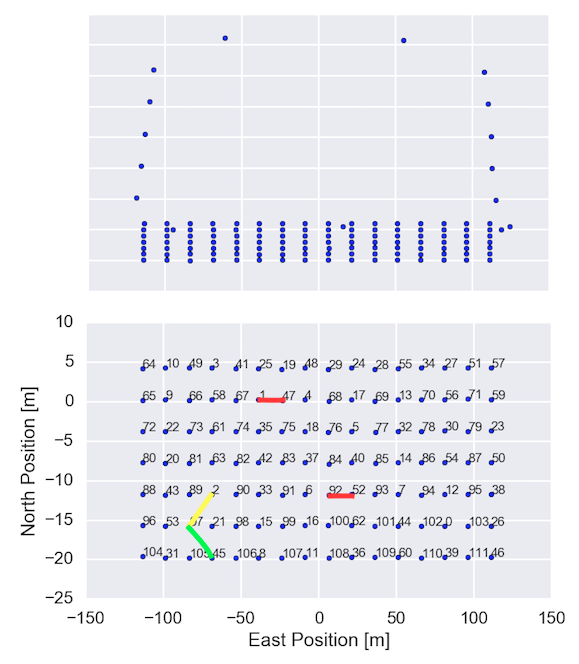
\includegraphics[width=\linewidth]{antpos128}

\caption{The PAPER-128 layout. Each dot corresponds to the location of
an antenna. Top panel shows the antenna positions drawn to scale;
bottom panel show the antenna labels and distances of the 112-element grid, in other words excluding the outrigger antennas.
The numbering of the antennas in the bottom panel are original labels
during instrument assembly and does not bear significant
meaning. In the bottom panel, the two baselines (5,77) and (40,85) marked with red segments are example of an equivalent pair, both with separation denoted by \{1,0\}, for the
antennas are separated by 1 unit east and 0 unit north. Similarly,
the baselines marked in blue and yellow are examples
of the classes \{1,1\} and \{1,-1\}, respectively. Due to the small North-South separation within the grid, \{1,1\} is expected to be near-equivalent to \{1,0\}. }
\label{fig:AntPos}
\end{figure}

We shall use the 128-element PAPER array (henceforth as PAPER-128) to motivate our formalism and demonstrate our method, and extend our results to several HERA configurations in Sec \ref{sec:arrconf}. 
The PAPER array is located in the Karoo desert in South Africa (30:43:17.5
S, 21:25:41.8 E). The layout pattern with antenna labels are show
in Fig. \ref{fig:AntPos}. The array consists of a 112-element grid and 16 "outriggers" used primarily to aid calibration.  In the bottom panel, the two baselines (5, 77) and (40, 85), marked in red, are an example of equivalent pair. We denote a equivalency-class of baselines in the PAPER grid by their separations, in this case  \{1,0\}, for the
antennas are separated by 1 unit east and 0 unit north. Similarly,
the baselines marked in blue and yellow are respectively examples
of \{1,1\} and \{1, -1\}.
Note \{1,0\} and \{-1, 0\} for example are the same class and should
not be counted twice. Antennas in purely north-south baselines
are close (4m), and hence these baselines are not suitable
for cross-multiplication due to cross-talks. On the other hand, the close North-South separation means that classes such as \{1,0\} and  \{1,1\} are expected to be near-equivalent. The PAPER-64 analysis of \cite{Ali2015} used three classes of baselines, the PAPER-128
equivalent of which are 
\{2, 0\}, \{2, 1\} and \{2, -1\}. There each of these classes
of baselines are cross multiplied within itself. This paper provides the method for inter-class multiplications. To do so we will use the short hand notation $\{m,n\}:\{m',n'\}$ to denote a pair of baseline classes to be cross-multiplied. 


\section{Method}

\subsection{Rough Idea \label{sec:tracks}}



Given a point source on the sky, each baseline maps to a point in $uv$ plane. As the Earth rotates with respect to
the source, the points trace out tracks in the $uv$ plane. 
We show in Fig. \ref{fig:Tracks} $uv$ tracks of PAPER-128 over 4.8 hours, at 0.15GHz, for a source that passes through zenith. 


\begin{figure}[H]
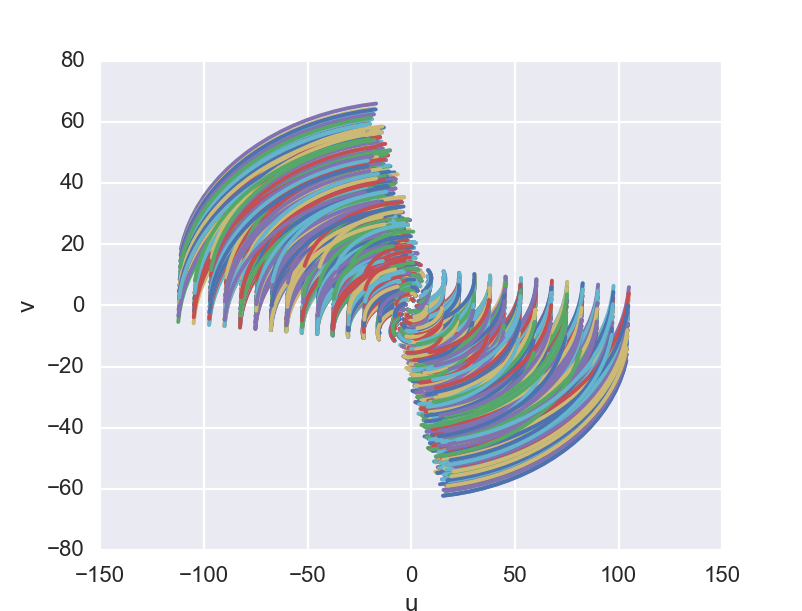
\includegraphics[width=\linewidth]{tracks128}
\caption{Tracks of PAPER-128 (grid only, excluding outriggers) for requency $\nu=0.15\text{GHz}$ and a hypothetical source that passes through zenith.
These tracks are traced out over 0.2 sidereal days, or roughly 4.8
hours. Color represents different baselines. 
As the Earth rotates, tracks are traced out counterclockwise. }
\label{fig:Tracks}
\end{figure}

Roughly speaking, we can identify
redundancy of near-equivalent baselines as crossings
of the $uv$ tracks. As we see in Fig. \ref{fig:Tracks}, there are many such crossings. However, crossing tracks do not imply perfect redundancy in the case of drift-scan arrays. In fact, track-crossing is
not accurate enough for time offset determination, nor can it give estimate of the degree of redundancy.  The reason lies in the finite size of the beams and the nature of a drift-scan measurement. This shall become evident in the next section, after we develop a more general formalism that accounts for the point spread function of the finite beams, and estimate the degree of redundancy for general combination of baselines at a general time-offset. We show sample beams of HERA and PAPER antennas in Fig. \ref{fig:Beam} for reference. 



\begin{figure}[H]
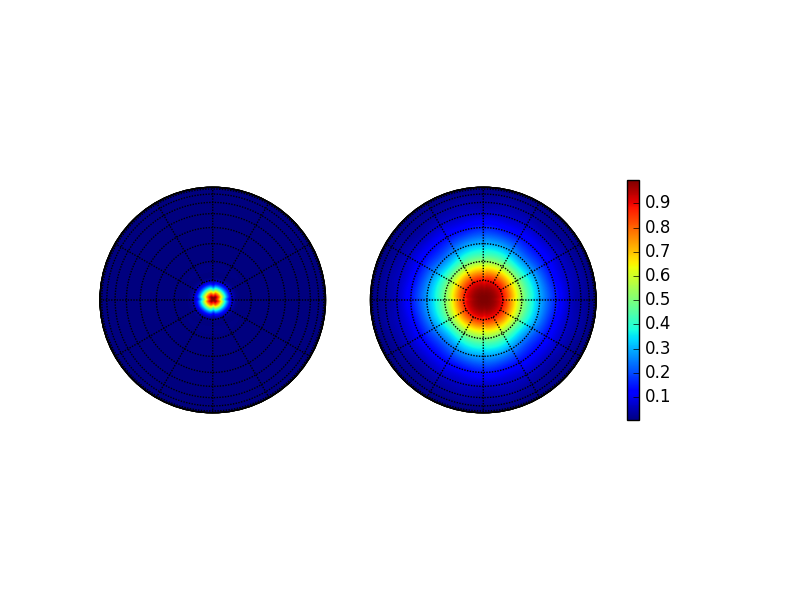
\includegraphics[width=1.2\linewidth]{Beams}

\caption{Example beam response of HERA (left) and PAPER (right) antennas. Both beams are Stokes $I$ polarization antenna voltage beams, at frequency of $\nu=150\text{MHz}$ and normalized to $1$ at zenith. Notice $A$ in this paper is a ``baseline's beam'', equivalent to squares of the antenna voltage beams shown here. The circles centered around zenith (center of beam) here are
spaced 10 degrees apart. \label{fig:Beam}}
\end{figure}



\subsection{Formalism}
In this section we formulate the relation between 
the product of visibilities from two arbitrary baselines and the power spectrum. 

We begin with the visibility as commonly defined in the literature (e.g.
\citealt{first-paper}): 
\begin{equation}
\begin{aligned}V_{\nu}(\boldsymbol{b}) & =\int d\Omega A_{\nu}(\hat{\boldsymbol{s}})\phi(\nu)I_{\nu}(\hat{\boldsymbol{s}})\exp\left(-2\pi i\frac{\nu}{c}\boldsymbol{b}\cdot\hat{\boldsymbol{s}}\right),\\
 & \approx\frac{2k_{B}}{\lambda^{2}}\int d\Omega A_{\nu}(\hat{\boldsymbol{s}})\phi(\nu)T(\hat{\boldsymbol{s}})\exp\left(-2\pi i\frac{\nu}{c}\boldsymbol{b}\cdot\hat{\boldsymbol{s}}\right),
\end{aligned}
\label{eq:Vis1}
\end{equation}
Here $k_B$ is Boltzmann's constant, $\lambda$ is the mean wavelength, $\boldsymbol{b}$ is the baseline
length, $\hat{\boldsymbol{s}}$ and $\Omega$ are a direction in the
sky and its corresponding solid angle. Inside the integral we have $\phi(\nu)$ the frequency bandpass profile, $A_{\nu}$ the (frequency
dependent) primary beam, and $I$ the specific intensity, which has been
related to $T$, the brightness temperature in the Rayleigh-Jeans
limit. The beam reception pattern $A$ is dimensionless,
normalized to 1 at its peak (zenith), and we assume it to be the same
for all baselines. In practice,
power spectrum measurements are typically taken from a few ten MHz centered around the corresponding redshift of interest (e.g. 150 MHz for z=9.5). Note that in Eq. \ref{eq:Vis1}, no flat-sky approximation has yet been made; the angular integral is performed over the dome. 

Delayed-transformed visibility has been widely adopted in recent years since it has been shown that foregrounds are isolated in delay space. We define the delay-transformed visibility by Fourier transforming visibility along the frequency axis\citep{delay-transform} as:
\small
\begin{equation}
\begin{aligned}V(\boldsymbol{b},\tau) & =\int d\nu V_{\nu}(\boldsymbol{b})\phi(\nu)\exp\left(-2\pi i\nu\tau\right),\\
 & =\frac{2k_{B}}{\lambda^{2}}\int d\Omega d\nu A(\hat{\boldsymbol{s}},\nu)\phi(\nu)T(\hat{\boldsymbol{s}},\nu)\exp\left[-2\pi i\nu\left(\frac{\boldsymbol{b}\cdot\hat{\boldsymbol{s}}}{c}+\tau\right)\right]. 
\end{aligned}
\label{eq:Vb1}
\end{equation}
\normalsize
Here the delay $\tau$ is the Fourier variable. Eq. \eqref{eq:Vb1} expresses the delay-transformed visibility as
an integral over observational coordinates $\hat{\boldsymbol{s}}$ and $\nu$. Ultimately,
we would like to relate the data, collected with coordinates $\hat{\boldsymbol{s}}$
and $\nu$, to the power spectrum, written with 
$\boldsymbol{r}$ and $\boldsymbol{k}$, the cosmological position coordinate and wavenumber. To do so, we start by noticing that
\[
\begin{aligned}r & =\frac{c}{H_{0}}\int_{0}^{z}\frac{dz'}{E(z')},\\
 & \approx\frac{c}{H_{0}}\int_{0}^{z_{0}}\frac{dz'}{E(z')}-\frac{c(1+z)^{2}}{\nu_{21}H_{0}E(z)}\left(\nu-\nu_{0}\right),\\
 & \equiv X-Y\Delta\nu,
\end{aligned} \label{eq:r}
\]
where $\nu_{21}=1420$MHz is the 21\,cm transition rest frequency, $\nu_{0}$
a reference central frequency with corresponding redshift $z_{0}$,
and 
\[
E(z)=\sqrt{\Omega_{m}(1+z)^{3}+\Omega_{\Lambda}}.
\]
Inverting for $\nu$:
\begin{equation}
\nu=\frac{X-r}{Y}+\nu_{21}.\label{eq:nur}
\end{equation}

Further we shall invoke the flat-sky limit, with the $z$ direction points to zenith, and $x$ and $y$ point east and north, respectively:
\begin{equation}
(r_{x},r_{y})=(X\hat{\boldsymbol{s}}_{x},X\hat{\boldsymbol{s}}_{y}). 
\end{equation}
In the same limit $(Xk_{x},Xk_{y},Yk_{z})=\frac{2\pi}{c}(b_{x},b_{y},\tau)$ relates
the cosmological $k$ to the observational coordinates. For a more rigorous treatment without the flat sky limit, see Appendix [ADRIAN]. 

We can rewrite the delayed-transformed visibility as 
\small
\[
\begin{aligned}V(\boldsymbol{b},\tau) & =\frac{2k_{B}}{\lambda^{2}}\int\frac{d^{3}r}{X^{2}Y}A(\boldsymbol{r})\phi(r)T(\boldsymbol{r})\exp\left[-2\pi i\left(\frac{\boldsymbol{b}}{c}\cdot\hat{\boldsymbol{r}}+\tau\right)\nu_{r}\right]\end{aligned},
\]
\normalsize
 where $d\nu=-dr/Y$ and $d^{3}r=-X^{2}Yd\Omega d\nu$. 
We have written $\nu_{r}$ as a reminder that $\nu$ and $r$ are related
by Eq. \eqref{eq:nur}. 

Most existing visibility based power-spectrum pipelines for redundant drift-scan  arrays relate the power-spectrum to the conjugate square of the visibilities \citep{first-paper, paper32, Ali2015}. We would like to generalize such relations by relating the power-spectrum to the product of two visibilities from two arbitrary baselines and time-offsets. 
The beam pattern of a baseline shifts relative to the sky as the Earth rotates. Here we choose to fix the sky, and denote the rotated coordinates
of the beam pattern with the 3 dimensional rotation operator $\Gamma$:
\small
\[
\begin{aligned}V(\boldsymbol{b'},\tau') & =\frac{2k_{B}}{\lambda^{2}}\int\frac{d^{3}r}{X^{2}Y}A(\Gamma\boldsymbol{r})\phi(r)T(\boldsymbol{r})\exp\left[-2\pi i\left(\frac{\boldsymbol{b}}{c}\cdot\Gamma\hat{\boldsymbol{r}}+\tau'\right)\nu_{r}\right]\end{aligned}.
\]
\normalsize
With implicit bounds of integrals from $-\infty$ to $\infty$, we have:
\begin{widetext}
\begin{equation}
\begin{aligned} & \langle V^{*}(\boldsymbol{b},\tau)V(\boldsymbol{b'},\tau')\rangle\\
 & =\left(\frac{2k_{B}}{X^{2}Y\lambda^{2}}\right)^{2}\int d^{3}rd^{3}r'\left(\langle T^{*}(\boldsymbol{r})T(\boldsymbol{r'})\rangle\right)A^{*}(\boldsymbol{r})A(\Gamma \boldsymbol{r'})\Phi_{b,\tau}(\boldsymbol{r},\Gamma \boldsymbol{r'}),\\
 & =\left(\frac{2k_{B}}{X^{2}Y\lambda^{2}}\right)^{2}\int d^{3}rd^{3}r'\left(\int\frac{d^{3}\kappa}{(2\pi)^{3}}\frac{d^{3}\kappa'}{(2\pi)^{3}}\langle T^{*}(\boldsymbol{\kappa})T(\boldsymbol{\kappa'})\rangle e^{-i(\boldsymbol{\kappa}\cdot \boldsymbol{r}-\boldsymbol{\kappa'}\cdot\boldsymbol{r'})}\right)A^{*}(\boldsymbol{r})A(\Gamma \boldsymbol{r'})\Phi_{b,\tau}(\boldsymbol{r},\Gamma \boldsymbol{r'}),\\
 & =\left(\frac{2k_{B}}{X^{2}Y\lambda^{2}}\right)^{2}\int d^{3}rd^{3}r'\left(\int\frac{d^{3}\kappa}{(2\pi)^{3}}P(\kappa)e^{-i\boldsymbol{\kappa}\cdot(\boldsymbol{r}-\boldsymbol{r'})}\right)A^{*}(\boldsymbol{r})A(\Gamma \boldsymbol{r'})\Phi_{b,\tau}(\boldsymbol{r},\Gamma \boldsymbol{r'}),\\
 & \approx\left(\frac{2k_{B}}{X^{2}Y\lambda^{2}}\right)^{2}P(k_{b,\tau})\int d^{3}rd^{3}r'\delta_{D}^{(3)}(\boldsymbol{r}-\boldsymbol{r'})A^{*}(\boldsymbol{r})A(\Gamma \boldsymbol{r'})\Phi_{b,\tau}(\boldsymbol{r},\Gamma \boldsymbol{r'}),\\
 & =\left(\frac{2k_{B}}{X^{2}Y\lambda^{2}}\right)^{2}P(k_{b,\tau})\int d^{3}r|A^{*}(\boldsymbol{r})A(\Gamma \boldsymbol{r})||\phi(\nu_{r})|^{2}\exp\left[-i2\pi\frac{\nu_{r}}{c}\left(\hat{\boldsymbol{r}}\cdot\boldsymbol{b}-\Gamma \hat{\boldsymbol{r}}\cdot\boldsymbol{b'}\right)\right],\\
 & =\left(\frac{2k_{B}}{\lambda^{2}}\right)^{2}P(k_{b,\tau})\int\frac{d\Omega d\nu}{X^{2}Y}|A^{*}(\hat{\boldsymbol{s}},\nu)A(\Gamma \hat{\boldsymbol{s}},\nu)||\phi(\nu)|^{2}\exp\left[-i2\pi\frac{\nu}{c}\left(\hat{\boldsymbol{s}}\cdot\boldsymbol{b}-\Gamma\hat{\boldsymbol{s}}\cdot\boldsymbol{b'}\right)\right],
\end{aligned}
\label{eq:main}
\end{equation}

where in transition from cosmological coordinates back to observing coordinates we have written $\hat{\boldsymbol{r}}\equiv\hat{\boldsymbol{s}}$, and 
\begin{equation}
\Phi_{b,\tau}(\boldsymbol{r},\Gamma \boldsymbol{r'})=|{\phi^{*}}(\ensuremath{\nu_{r}})\phi(\nu_{r'})|\exp\left[-i\frac{2\pi}{c}\left(\boldsymbol{b}\cdot\nu_{r}\hat{\boldsymbol{r}}-\boldsymbol{b'}\cdot\nu_{r'}\Gamma\hat{\boldsymbol{r'}}\right)\right]\exp\left[-i2\pi\tau\left(\nu_{r}-\nu_{r'}\right)\right].
\end{equation}
\end{widetext}
The third equality of Eq.(\ref{eq:main}) follows from assumption of translational invariance of sky statistics, and the first inequality follows from the assumption that
the 3D power spectrum varies negligibly over the $k$-space of interest
so that $\hat{P}_{21}(k+k')\approx\hat{P}_{21}(k)$. Since $\Gamma$
is a sky rotation, it does not affect $\nu$, hence we have taken $\nu_{r}$
outside the parenthesis in the phase term $\exp\left[-i2\pi\frac{\nu_{r}}{c}\left(\hat{\boldsymbol{r}}\cdot\boldsymbol{b}-\Gamma \hat{\boldsymbol{r}}\cdot\boldsymbol{b'}\right)\right]$. Notice that the phase factor $\exp\left[-i2\pi\tau\left(\nu-\nu'\right)\right]$
drops out in the end. This means that the location and magnitude of the correlation peak does not depend on delay $\tau$, an important point we shall come back to. 

Since the beam pattern and bandwidth are given in $\hat{\boldsymbol{s}}$
and $\nu$, we convert the integral back to these coordinates to get
the general relation between the delay-transformed visibilities and
the power spectrum:

\begin{equation}
\begin{aligned} & \langle V^{*}(\boldsymbol{b},\tau)V(\boldsymbol{b'},\tau')\rangle\\
 & =\left(\frac{2k_{B}}{\lambda^{2}}\right)^{2}P(k_{b,\tau})\int\frac{d\Omega d\nu}{X^{2}Y}|A^{*}(\hat{\boldsymbol{s}},\nu)A(\Gamma\hat{\boldsymbol{s}},\nu)||\phi(\nu)|^{2}\\
 & \qquad \qquad \qquad \qquad \exp\left[-i2\pi\frac{\nu}{c}\left(\hat{\boldsymbol{s}}\cdot\boldsymbol{b}-\Gamma\hat{\boldsymbol{s}}\cdot\boldsymbol{b'}\right)\right].\end{aligned}
\label{eq:final}
\end{equation}

In other words the power spectrum estimate from visibilities of a baseline pair is given by 
\begin{equation}
 P(k_{b,\tau}) = \left(\frac{\lambda^{2}}{2k_{B}}\right)^{2} \frac{\langle V^{*}(\boldsymbol{b},\tau)V(\boldsymbol{b'},\tau')\rangle}{\Theta}, 
 \label{eq:opp}
\end{equation}
where the weight
\begin{equation}
\Theta \equiv\int d\nu \Theta_{\nu}, 
\label{eq:Theta}
\end{equation}
and 
\[
\Theta_{\nu}\equiv \int \frac{d\Omega}{X^{2}Y}|A^{*}(\hat{\boldsymbol{s}},\nu)A(\Gamma\hat{\boldsymbol{s}},\nu)||\phi(\nu)|^{2} e^{-i2\pi\frac{\nu}{c}\left(\hat{\boldsymbol{s}}\cdot\boldsymbol{b}-\Gamma\hat{\boldsymbol{s}}\cdot\boldsymbol{b'}\right)}e^{i\psi}.
\label{eq:Thetanu}
\]
Notice that $\Theta$ has no dependence on $\tau$. In Eq. \ref{eq:Thetanu} we introduced an extra phase $\psi$, the origin of which we shall explain in \ref{sec:rephs}. 

Roughly speaking, Eq. \ref{eq:opp} through \ref{eq:Thetanu} tell us that the cross multiplications of visibilities at a time delay
in $uv$-space is proportional to the power spectrum times the Fourier
transform of the cross multiplied beam pattern. As a check, when applied to equivalent baselines,
$\boldsymbol{b}=\boldsymbol{b'}$, $\hat{\boldsymbol{s}}=\Gamma\hat{\boldsymbol{s}}$, and Eq.(\ref{eq:final}) reduces to Eq.(B9) of \cite{paper32}. 
With Eq. \ref{eq:opp} and Eq. \ref{eq:Theta} we can, for any given pair of baseline classes and time delay, estimate the degree of redundancy, here represented by $\Theta$, thereby achieving all our goals stated in the introduction, i.e. to identify 
candidate baseline pairs with good redundancy, to find the time offset that maximizes redundancy, and to quantify the degree of such redundancy. We can do all the above simply by computing the weight $\Theta$ from
Eq.(\ref{eq:Theta}) for various time offsets, without having to actually cross-multiply visibilities for all baselines and offsets. This makes the task computationally tractable. 

\section{Analysis}

\subsection{Track-crossing, beam, and phase}
We are now in a position to understand the reason that track-crossing, as mentioned section \ref{sec:tracks}, does not correspond exactly to the peak of correlation. Typical convention of rotation synthesis has rotation operates on $\boldsymbol{b'}$ instead of $\hat{\boldsymbol{s}}$, in which case Eq.\ref{eq:Theta} becomes
\begin{equation}
\Theta \equiv\int\frac{d\Omega d\nu}{X^{2}Y}|A^{*}(\hat{\boldsymbol{s}},\nu)A(\Gamma\hat{\boldsymbol{s}},\nu)||\phi(\nu)|^{2} e^{-i2\pi\frac{\nu}{c}\hat{\boldsymbol{s}}\cdot\left(\boldsymbol{b}-\widetilde{\Gamma}\boldsymbol{b'}\right)}, 
\end{equation}
where $\widetilde{\Gamma}$ is the inverse of $\Gamma$. Track-crossing corresponds to vanishing of the exponent
\[
 \boldsymbol{b}-\widetilde{\Gamma}\boldsymbol{b'} = 0. \label{eq:trackcross}
 \]
This condition maximizes $\Theta$ if and only if no other term in the integral depends on $\Gamma$, i.e. if and only if $A(\Gamma\hat{\boldsymbol{s}},\nu)=A(\hat{\boldsymbol{s}},\nu)$. If the measurement is tracking, $\Gamma$ becomes a rotation around zenith, and the condition is satisfied. In a general drift-scan measurement, this is not the case, and track-crossing point of Eq. \ref{eq:trackcross} does not maximize $\Theta$. 

\begin{figure}[h]
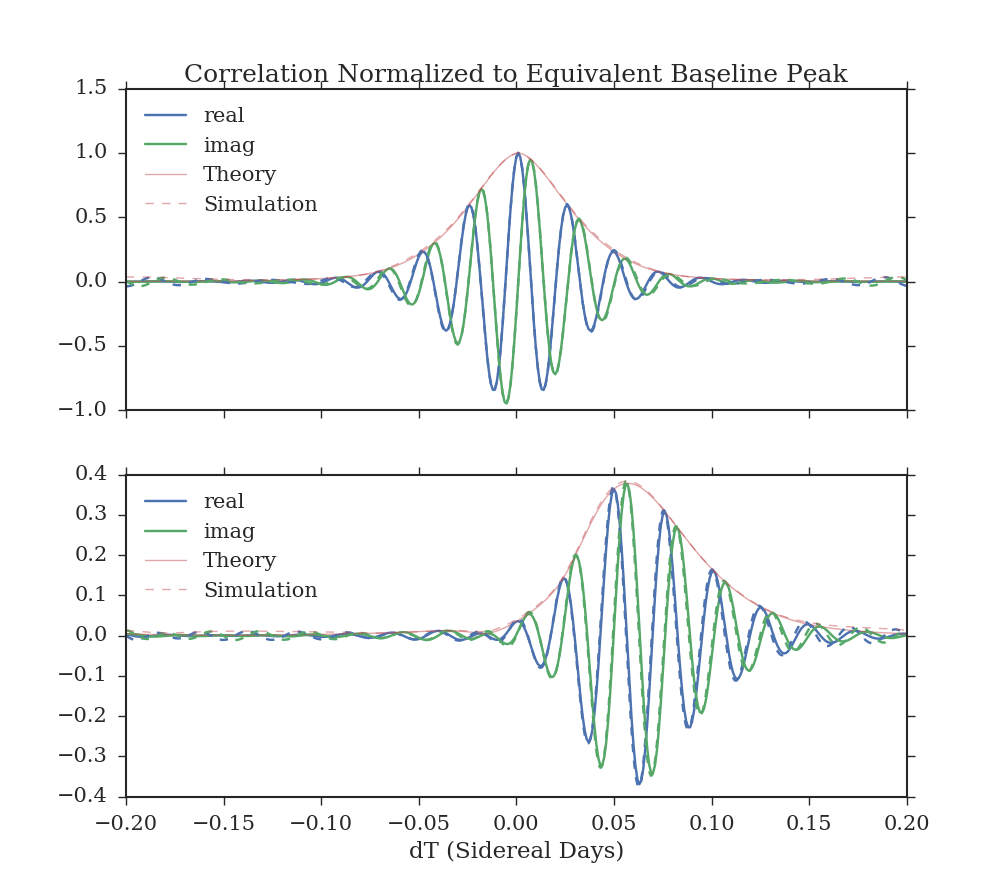
\includegraphics[width=\linewidth]{opp}

\caption{Numerical comparisons of the visibility correlation peaks to the $\Omega$ factor in Eq.(\ref{eq:final}). We generated 2500 instances of Gaussian random sky on healpix maps, computed visibilities and cross correlated them to find the correlation.  Top panel shows the equivalent baseline pairs \{1,0\} against \{1,0\}, bottom panel shows set1,0 against \{1,1\}.  Evaluations of weight $\Theta$ are shown with solid curves, and the visibility correlations of simulated random sky is given with dashed lines. In both cases blue denotes real part, green the imaginary part, and red the magnitude. We see that in both cases the theory and simulation line up in both amplitude and phase.}
\label{fig:numerics}
\end{figure}

We shall illustrate with an example from PAPER128. In the solid curves of Fig. \ref{fig:numerics} we show examples of $\Theta_{\nu}$ as a function of time offset  here with no additional phase. The amplitude and real, as well as imaginary parts are shown for equivalent \{1,0\}:\{1,0\} in the top panel, and near-equivalent \{1,0\}:\{1,1\} in the bottom. The vertical axis is normalized such that the peak of \{1,0\}:\{1,0\} is unity. We see that as expected, \{1,0\}:\{1,0\} peaks at $dT=0$, where $\Theta_{\nu}$ is real. \{1,0\}:\{1,1\} on the other hand, peaks with amplitude of approximately 0.4 at $dT\approx0.055$ days and is not real at its peak. Since track-crossing corresponds to vanishing exponent, correlation at track-cross points are real. This in the bottom plot corresponds to roughly $dT=0.05$ days. 

Shown in dashed curves, which almost completely overlap with the solid curves, in Fig. \ref{fig:numerics} are cross-multiplications of simulated visibilities. For the simulation, we take N=2500 random realizations of the sky
on a healpix map \citep{Heal, HealPrimer} \footnote{We use functionalities in the python package AIPY for healpix mapping
as well as coordinate transforms. }, and pick two baselines \{1,0\} and \{1,1\}. For each realization, each pixel is given a Gaussian random value
of brightness temperature. We then rotate the baseline positions with
the appropriate rotation matrix, multiplying the sky by the primary beam to get the visibilities, for each
baseline\footnote{There are two obvious ways to achieve the rotation. One
can either fix the sky and rotate the baselines, or the other way
around. We found however, that we must not physically rotate the sky
map, for the numerical round-offs due to finite resolutions of the
map turns out to be significant. Thus we let the sky, represented
by the healpix map, be fixed, and rotate the baselines. }. The resulting visibilities for the two baselines are then convolved
via the Fourier convolution theorem, to obtain values of the cross
correlation as a function of time-offset. The peak of the curve then
corresponds to maximum redundancy.  We do this for both the equivalent (\{1,0\}:\{1,0\}) and near-equivalent (\{1,0\}:\{1,1\}) case.



\subsection{Rephasing \label{sec:rephs}}
As we see in Fig.\ref{fig:numerics}, $\Theta$ at the peak of correlation is in general complex, and often far from real. Furthermore, this phase of peak correlation is inevitably frequency dependent, as we see in Eq. \ref{eq:Thetanu}. This frequency dependence of the phase would lead to destructive interference when we integrate over frequency, unless we correct one of the visibilities by an extra phase $\psi_\nu$. 

The physical origin of $\psi_\nu$ lies in the two visibilities having different phase centers. By default the correlators of a drift-scan array phase the two visibilities both to zenith at the same time. When they are cross-multiplied with a time lag, they must be rephased to the account for the movement of the zenith. Thus in practice we must rephase the visibilities before delay transform. 
%Doing so is also crucial to reduction of additional mode mixing, as discussed in \cite{Hazelton2013}. Shapes of overlapping regions of pairs of baselines are fixed with respect to frequency. 


In Fig. \ref{fig:freqdiff} we compare the cross-multiplied visibilities of both equivalent and near-equivalent baseline pairs for two channels: 0.16 GHz and 0.17 GHz. The top two panels have zero rephasing, and the bottom two are rephased to a time offset of 0.055 sidereal days, the optimal time offset for the given baseline pair. The first and third panels show the equivalent baseline pairs \{1,0\}:\{1,0\}, and second and fourth panels show \{1,0\}:\{1,1\}. We see that in the un-rephased case in the second panel, although the magnitude of correlations match up for the two frequencies, the phases do not. This means summing over frequency leads to destructive interference and signal loss. The wider the frequency profile, the more destructive the interference would be. In the rephased case, the phases of the near-equivalent case match up and can be added without compromising sensitivity. We should thus rephase the data separately for each set of baseline pairs. 

\begin{figure}[H]
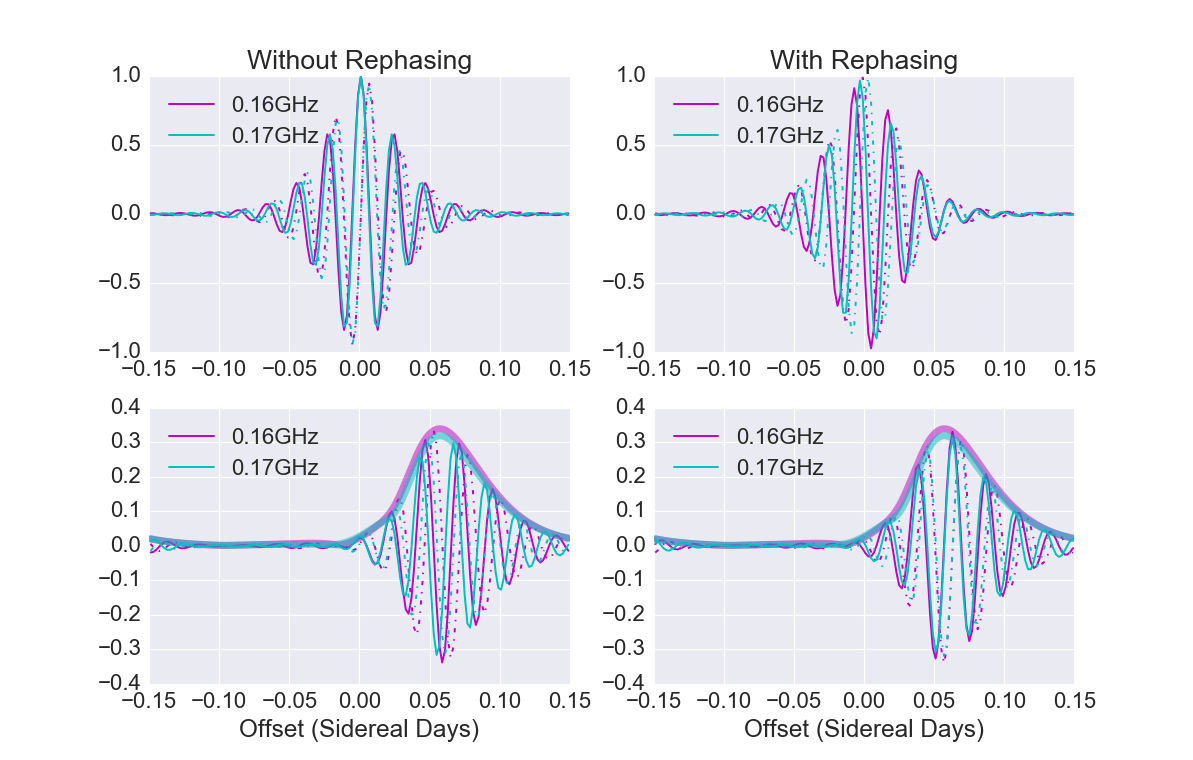
\includegraphics[width=1.1\linewidth]{rephs}

\caption{Comparisons of the peak phases of two different frequencies. Specifically shown are the real parts of $\Theta_{\nu}$. First and third panels shows equivalent baselines, second and fourth show a pair of near-equivalents. The top two panels have zero phase shift ($\psi_{\nu}=0$), and the bottom two are rephased to a time offset of 0.055 sidereal days. The first and last panels thus show a coherently rephased series that would add constructively at the respective peaks. }
\label{fig:freqdiff}
\end{figure}

Once rephased, the overall weight can be constructed by $\Theta=\int \Theta_{\nu}d\nu$. We must numerically check that rephasing the weight as in Eq.\ref{eq:Thetanu} is indeed equivalent to rephasing the input visibilities before delay-transform. In other words, we want to verify that 
\begin{equation}
\begin{aligned} & \langle V^{*}(\boldsymbol{b},\tau)V_{\psi}(\boldsymbol{b'},\tau')\rangle\\
 & =\left(\frac{2k_{B}}{\lambda^{2}}\right)^{2}P(k_{b,\tau})\int\frac{d\Omega d\nu}{X^{2}Y}|A^{*}(\hat{\boldsymbol{s}},\nu)A(\Gamma\hat{\boldsymbol{s}},\nu)||\phi(\nu)|^{2}\\
 & \qquad \qquad \qquad \qquad \exp\left[-i2\pi\frac{\nu}{c}\left(\hat{\boldsymbol{s}}\cdot\boldsymbol{b}-\Gamma\hat{\boldsymbol{s}}\cdot\boldsymbol{b'}\right)\right].\end{aligned}
\label{eq:final}
\end{equation}


\subsection{Numerical Test \label{sec:Techniquet}}

First we present some numerical tests of our formalism to verify the validity of using $\Theta$ to estimate the degree of redundancy as a function of time lag. To do so, we need to compare the amplitude and phase of the integral weight $\Theta$ 
for a pair of baselines with products of simulated visibilities of those baselines. For computational simplicity, we shall use a single frequency channel of $150$MHz for the comparison. We may use this simplification without compromising generality because Eq. (\ref{eq:final}) is valid for a range of frequency channels if and only if it's valid for each single channels, provided that different channels are combined with rephasing as described in Sec. \ref{sec:rephs}. 

 The accuracy of this result is
limited by (simulated) cosmic variance and finite spacial resolution,
and hence can be beat down by averaging over a large number of universes.
A numerical estimate of the error of the peak height with $N=1$ is
$\lesssim20\%$, and thus with $N=2500,$ we achieve an error of peak
height $<0.5\%$. 




The comparison is show in Fig. \ref{fig:numerics}. 
Sensitivity contribution is inferred from height of the peak of the cross-multiplied visibilities as a function of time. 
We first compare the simulation to the analytical weight $\Theta$ for a pair of equivalent baselines (\{1,0\}, \{1,0\}), then normalize the peaks 
of the near-equivalent baselines (\{1,0\}, \{1,1\}) to that of the equivalent ones. 
In Fig. \ref{fig:numerics}  we show on the top comparison of
the convolution of an equivalent baseline of PAPER-128, normalized to 1 at the
peak, whose location is at zero time offset as expected. On the bottom we show
comparison of a near-equivalent baseline pair, of classes \{1,0\}:\{1,1\} and \{1,1\}:\{1,1\}. The peaks
are normalized with the same factor as the peak height on the top,
i.e. the two plots have thus the same scale on the vertical axis.
The height of the plot thus quantifies the added sensitivity. We see at a peak of around 0.055 sidereal days, or 1.32 hours, the two baselines are maximally redundant. 




At the optimal time separation, the integral in Eq. \eqref{eq:final}
is maximized. Thus as another check we expect the two beams to have to same fringe pattern
(frequency and phase). Due to the time delay, however, the beam center
would be slightly shifted with respect to each other. This we show
in Fig. \ref{fig:Beam-fringe-pattern}. The left and middle panels show the beam fringe
patterns for baselines \{2,0\} and \{2,1\}, delayed by 0.0325 sidereal days,
and the right panel shows their cross product. The fringe pattern
indeed cancels out as we expect. 


\begin{figure*}[h!]
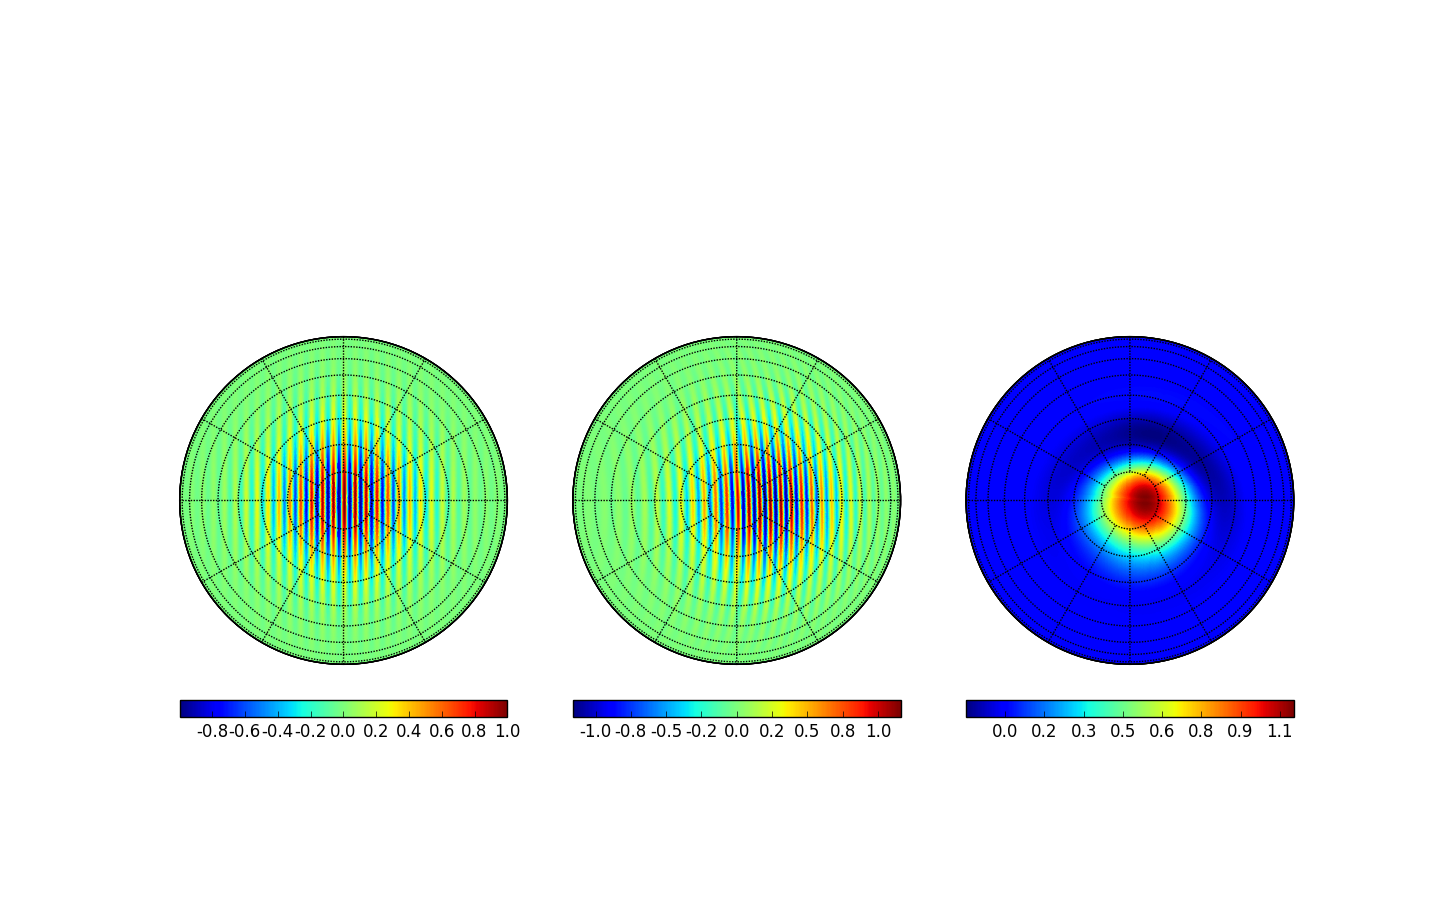
\includegraphics[width=0.9\textwidth]{fringe_res}
\caption{Beam fringe pattern of \{2,0\}(left), \{2,1\} at a time delay (middle),
and their conjugate product (right). Frequency of $\nu=0.15\text{GHz}$ is
chosen and only the real components are shown. The colorbar values are normalized such that the peak of the original beam is 1. \label{fig:Beam-fringe-pattern}}
\end{figure*}



\begin{figure*}[h!]
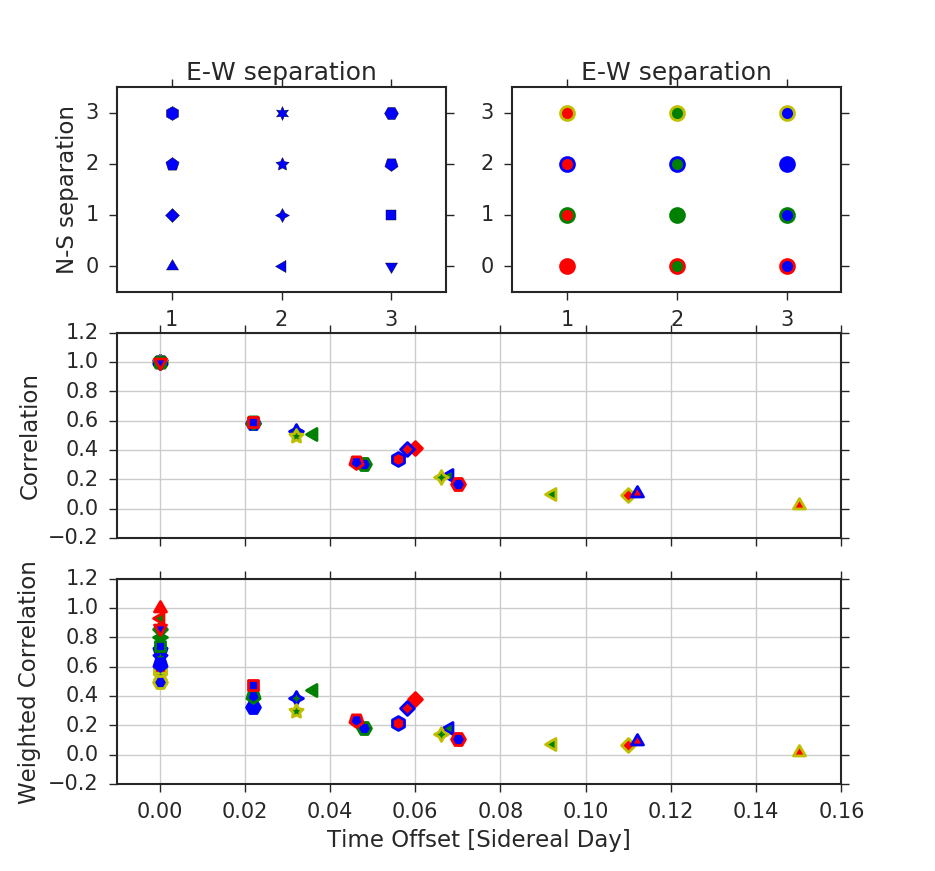
\includegraphics[width=\textwidth]{sensitivity_1}

\caption{Relative sensitivity contributions of selected baseline combinations in PAPER-128. In the legend m,n:p,q denotes cross
multiplying PAPER-128 baselines of east-west, north-south separations (m,n) and (p,q) respectively. The top
panel shows the peak height (degree of correlation) of each baseline
combination, while the bottom panel multiplies the heights by the
corresponding multiplicities as in Eq. \eqref{eq:sensul}. 
In weighting by the multiplicity (bottom), we have chosen to fix the sensitivity 
contribution of 1,0:1,0 to unity. The same symbols and colors correspond in the top and bottom panel, with half of the legend shown in each. }
\label{fig:sensplot}
\end{figure*}

\begin{figure*}[h!]
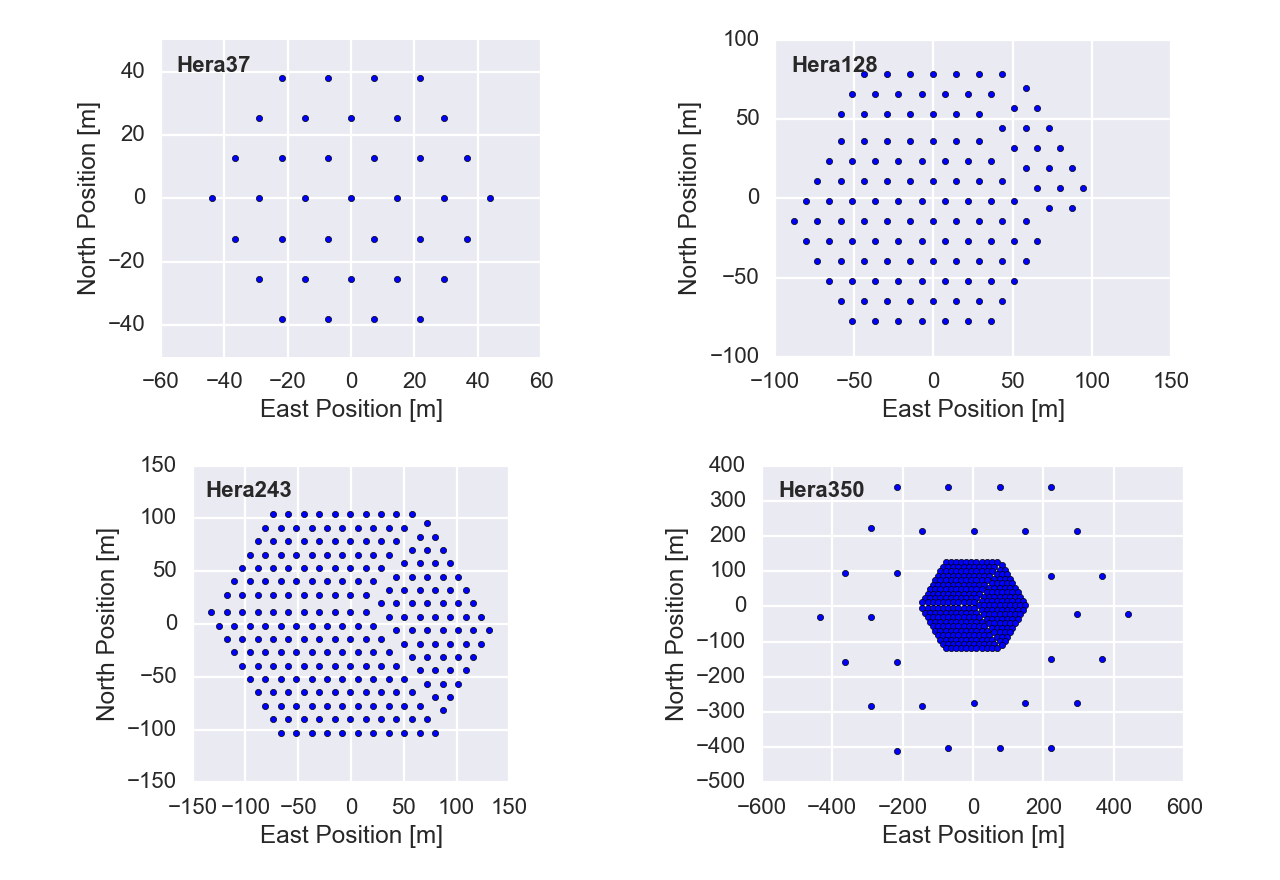
\includegraphics[width=0.9\textwidth]{HeraAntpos}
\label{fig:HeraAntpos}
\caption{Planned Hydrogen Epoch of Reionization Array antenna configurations. HERA 37 is expected to complete and start collecting data in summer of 2017, and the other three are planned configurations in the next phases. For HERA350, only the 320 elements in the core are shown. }
\end{figure*}

\subsection{ Sensitivity \label{sec:sensitivity}}

Having verified Eq. \eqref{eq:final}, we can thus predict the sensitivity contributions of a
particular baseline pair simply by computing the integral Eq. \.
Intuitively we expect the sensitivity to depend on both the $uv$ coverage of the baseline and the patch of sky inside the beam. A larger beam like that of PAPER would tolerate larger time-offsets because more sky area can coincide in the two beams \footnote{Larger beams also imply smaller spread in $uv$ space. This could lead to either larger or smaller redundancy, which depends on the overlap of two such point spread functions.}
Having computed all of the baseline pairs, we find that baseline pairs that are mirror images of each other 
give the same amount of redundancies (peak height), with the opposite time offset, as expected from symmetry. 
For example, \{1,0\}:\{1,1\} is mirror image of \{1,0\}:\{1,-1\} and these two baseline pairs
give the same sensibility contribution. Thus we shall only show a subset of representative baseline pairs to illustrate the contributions from different classes of baseline pairs. For a more complete result see Fig. \ref{fig:pairplot}.  

In the top panel of Fig. \ref{fig:sensplot}
we show the peak heights and locations for a variety of baseline combinations.
We see that baseline pairs that have crossings at a smaller time delay
tend to have higher correlations. In other words, correlation peaks
that are closer to zero time lag are higher. This is expected since
a) the longer the time delay, the more the antennas have moved with respect
to the sky and hence the less overlaps in patch of sky surveyed, b) smaller optimal
time-offset corresponds to smaller differences in orientation and length of the 
pair of baselines. 




To determine that actual relative contribution to sensitivity of these
baseline pairs, we have to take into account of the multiplicities of
these baselines. By these we mean how many physical antenna pairs have the
same length and orientation. Looking at Fig. \ref{fig:sensplot}
we see for example \{1,0\} will have higher multiplicity than \{2,0\},
or \{1,1\}. The latest release of PAPER-64 data uses the 128-equivalent baselines \{2,1\},
\{2,0\} and \{2,-1\} \citep{Ali2015}, and achieved a $2\sigma$ upper
limit of $(22.4\text{mK})^{2}$. There, the three sets of equivalent baselines
are only cross multiplied by itself. Assuming that each baseline delivers
the same quality of data (meaning they have the same height of correlation
peaks, which is in our normalization equal to unity), the relative
contribution to sensitivity can be estimated. 

First we can average of the visibilities of the equivalent baselines. Since the core of PAPER-128 has 16 by 7 antenna configuration, there
are $M\equiv(16-|m|)\times(7-|n|)$ copies of the baseline class $\{m,n\}$. This means
that if we add visibility measurements of all these equivalent baselines,
we get a factor of $\sqrt{M}$ reduction in noise
level $\sigma_N$ of the visibility. The sensitivity contribution of $\{m,n\}$, cross multiplied with $\{m',n'\}$  thus roughly speaking scales as $\sqrt{\left((16-|m|)(7-|n|)(16-|m'|)(7-|n'|)\right)}=\sqrt{MM'}$.
For cross-multiplications of near-equivalent baselines of
types $\{m,n\}$ and $\{m',n'\}$, we get an effective weight: 

\begin{equation}
\widetilde{\Theta}_{bb'} \propto \Theta_{bb'}\times\sqrt{MM'}.\label{eq:sensul}
\end{equation}

Shown in the bottom panel of Fig. \ref{fig:sensplot} is the peak heights weighted
by the multiplicity factor. Points that have zero time delay are the equivalent baseline pairs and their weighted correlation values simply reflect the multiplicity factor. For clarity of presentation we have ``folded over'' the negative time delays and combined baseline pairs that are identical modulus parity. We point out that the data points shown here are not all the cases of highest correlation.  




Having defined the modified weight $\widetilde{\Theta}$, we can estimate the power spectrum by inverse covariance weighting:
\begin{equation}
\begin{aligned}
 P(k_{\tau}) &= \frac{\sum_{bb'}P(k_{b,\tau})/\sigma_P^2(bb')}{\sum_{bb'}\sigma_P^2(bb')}, \\
 &= \frac{\sum_{bb'}P(k_{b,\tau})\widetilde{\Theta}_{bb'}^2}{\sum_{bb'}\widetilde{\Theta}_{bb'}^2},
 \end{aligned}
\end{equation}
where the sum is over classes of baseline pairs. 
We define the estimator sensitivity to be the inverse of the power spectrum noise variance:
\begin{equation}
\rho \propto \frac{1}{\sigma_P^2} \propto \rho_0^2\sum_{bb'}^N\widetilde{\Theta}^2_{bb'},
\end{equation}
where, if $\sigma_S^2$ and $\sigma_N^2$ are the characteristic signal and noise levels of a single-baseline visibility, $\rho_0\equiv\sigma_S^2/\sigma_N^2$ is the signal to noise ratio. 


The scaling in Eq. \ref{eq:sensul} was rough for simplicity of motivation. As we derive in Appendix \ref{sec:appB}, this weight should be corrected by a factor proportional $\rho_0$:

\begin{equation}
\label{eq:tildereal}
\widetilde{\Theta}_{bb'}=\frac{\Theta_{bb'}\sqrt{M_bM_{b'}}}{\sqrt{1 + \rho_0 \left(M_b+M_{b'} \right)}}.
\end{equation}

For a given $\rho_0$ Eq.\ref{eq:tildereal} thus quantifies the relative sensitivity contribution of a baseline pair $bb'$. Assuming a reionization signal of $\Delta_{21cm}^2\sim 30mK^2$, observation at 150MHz ($z=8.5$), 120 days of observation with PAPER antennas, we have roughly
(See Eq.(20) in \cite{first-paper})
\begin{equation}
\rho_0 \sim 0.001\left[\frac{L}{40m}\right] \left[\frac{0.1hMpc^{-1}}{k}\right]^3, 
\end{equation}
where $L$ is the baseline length. We only need a single characteristic $L$ even in the near-equivalent case because only baselines of nearly equal length would have high redundancy.As expected, baseline-pairs that have smaller $\widetilde{\Theta}$ contribute less to the sensitivity. 

\subsection{Array Configuration Comparisons \label{sec:arrconf}}
We run our algorithm over all possible baseline-pairs of  PAPER128, HERA37, HERA128, HERA243 and HERA350. The HERA antenna configurations are shown in Fig. \ref{fig:HeraAntpos}. The  
hexagonal design is the densest pattern of antenna-packing. The larger arrays are designed with a ``gap'' dividing the antennas into three different regions. The gaps are designed so as to improve $uv$ coverage and ease calibration without compromising sensitivity, but also produces many more near-equivalent baselines than the versions without the gap. The motivations behind the designs are explained in \cite{HERAconfiguration}.  The lack of short baselines that are visually close to each other, as well as the smaller beam (Fig. \ref{fig:Beam}) means that we expect to see only longer near-equivalent baselines. The lower multiplicities per class of baselines is made up with the larger number of classes of baseline-pairs, especially given the gap in the larger versions. 

\begin{figure}[H]
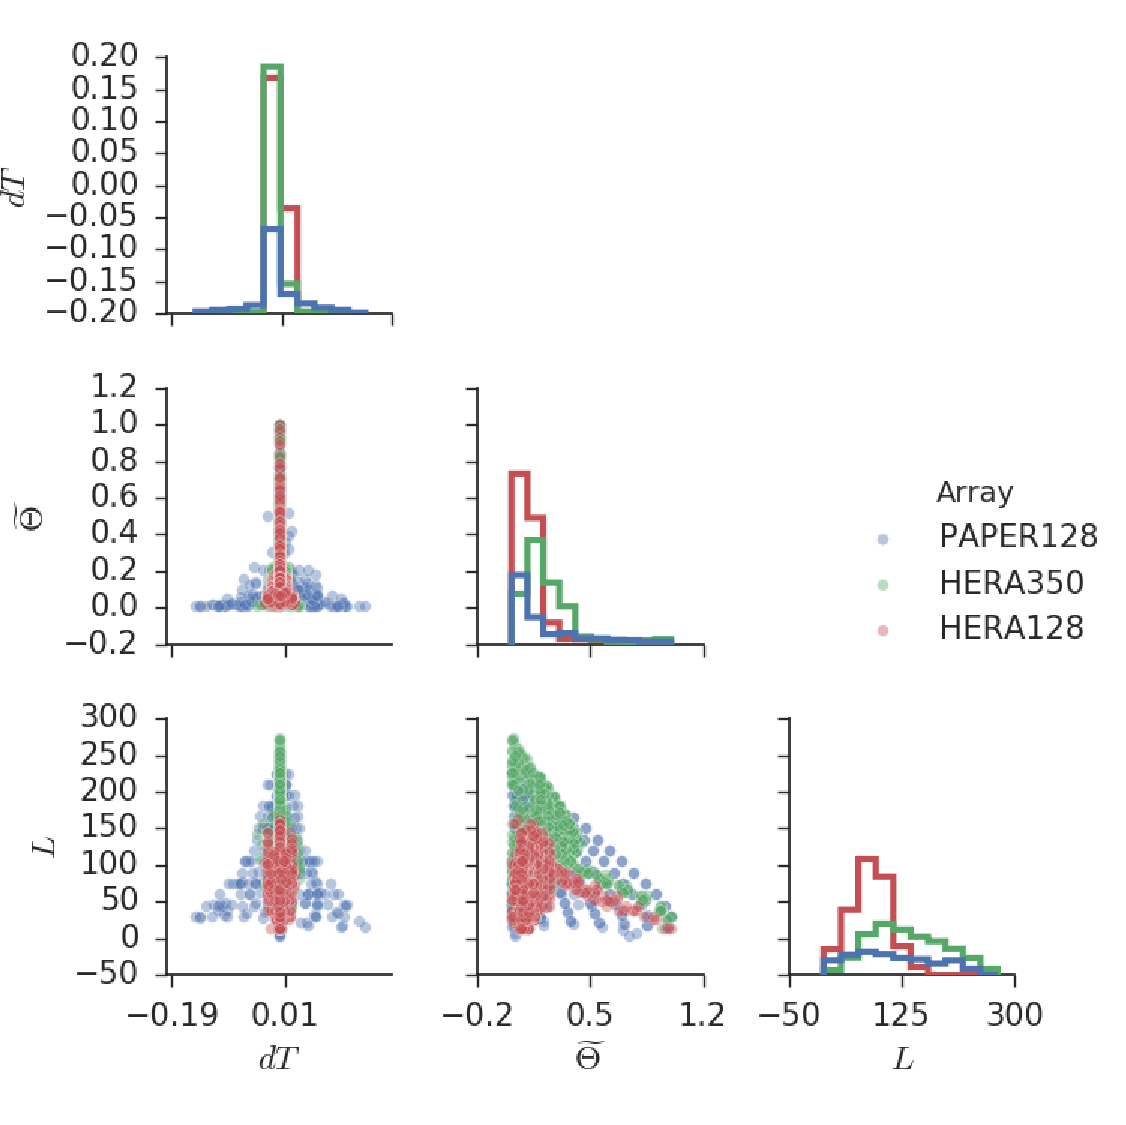
\includegraphics[width=\linewidth]{pairplot_small}

\caption{Pairplots of the top contributing baseline pairs in three arrays. Plotted properties are optimal time delay $dT$,  effective weight $\widetilde{\Theta}$ and baseline length $L$. Only those points with $\widetilde{\Theta}>0.01$ are shown (the weight for the top class of equivalent pair is normalized to 1). Only one baseline length is shown since all top contributing pairs have very similar lengths as expected. The scatter plots are shown with transparency so that darker regions indicate degeneracies. Scatter points of the 3 arrays overlap, in order indicated by the legend. }
\label{fig:pairplot}
\end{figure}

In Fig. \ref{fig:pairplot} we present a paired distribution of 3 different properties for baselines that contribute well to the sensitivity ($\widetilde{\Theta}>0.01$, where again the weight for the top class of equivalent pair is normalized to 1). The $dT$ vs. $\widetilde{\Theta}$ plot is familiar from Fig. \ref{fig:sensplot}. We only show 3 of the mentioned arrays for visual clarity. The other two results are similar barring intuitive differences. We make a few observations:
\begin{itemize}

\item Mapping of equivalent baseline pairs: the equivalent baselines are located in key points in the plots. They are the vertical bars in the lower left four plots and the highest peak in the first three histograms, the upper "diagonal edge" in the $\widetilde{\Theta}$ vs. $dT$ and the linear trend in the $\widetilde{\Theta}$ vs. $L$ plot for HERA arrays . 


\item Longer baselines roughly peak at lower time-offset, and lower multiplicity. This is intuitive for PAPER since  for the same north-south separation the rotation angle is smaller with longer east-west separation. 

\item The top near-equivalent pairs in HERA the same $\Theta$ (not shown) as in PAPER128, but much lower $\widetilde{\Theta}$. This is because they are longer baselines with lower multiplicity. In the end these baseline classes still lead to high contributions to total sensitivity (Fig. \ref{fig:osens}) because there are a lot more such baseline pairs for HERA.  

\end{itemize}

Having quantified the sensitivity from a given pair of baselines, we study the cumulative sensitivity of the array depending on which baseline pairs we include. Evidently we should prefer the pairs with larger $\widetilde{\Theta}$. In Fig. \ref{fig:osens} we plot $\rho$ against the minimum $\widetilde{\Theta}$. $\rho(\widetilde{\Theta}_{min})$ is the sensitivity of the array when baseline-pairs that have $\widetilde{\Theta}>\widetilde{\Theta}_{min}$ are included. The dashed lines represent the values when only the equivalent baseline-pairs are used.  We see as expected that in all cases using the near-equivalent baselines lead to more and more significant improvements with lower $\widetilde{\Theta}_{min}$, or in other words when worse baseline pairs are used. The small HERA37, with no gap (like in HERA350) or short near-equivalent baselines (like in PAPER 128), will not benefit much from the near-equivalent baselines. The maximum benefits for other cases are expected to be around $20\%$ to $60\%$. PAPER128 is designed with highly redundant near-equivalent baselines, and thus  these baselines start contributing at higher $\widetilde{\Theta}_{min}$, but the gapped HERA configurations will benefit even more from near-equivalent baselines at low $\widetilde{\Theta}_{min}$ due to there being more classes of such pairs. Note that here we normalized $\rho$ such that the contribution of the top equivalent baseline pair, such as (sep0,1:0,1 in the PAPER128 case) are 1. This plot therefore does not compare the absolute sensitivity across the different arrays. The stepwise pattern is characteristic of a regular grid; as we step to lower $\widetilde{\Theta}$ large groups of baseline pair classes get included in ``batch''. 
%\begin{centered}
\begin{figure}[H]
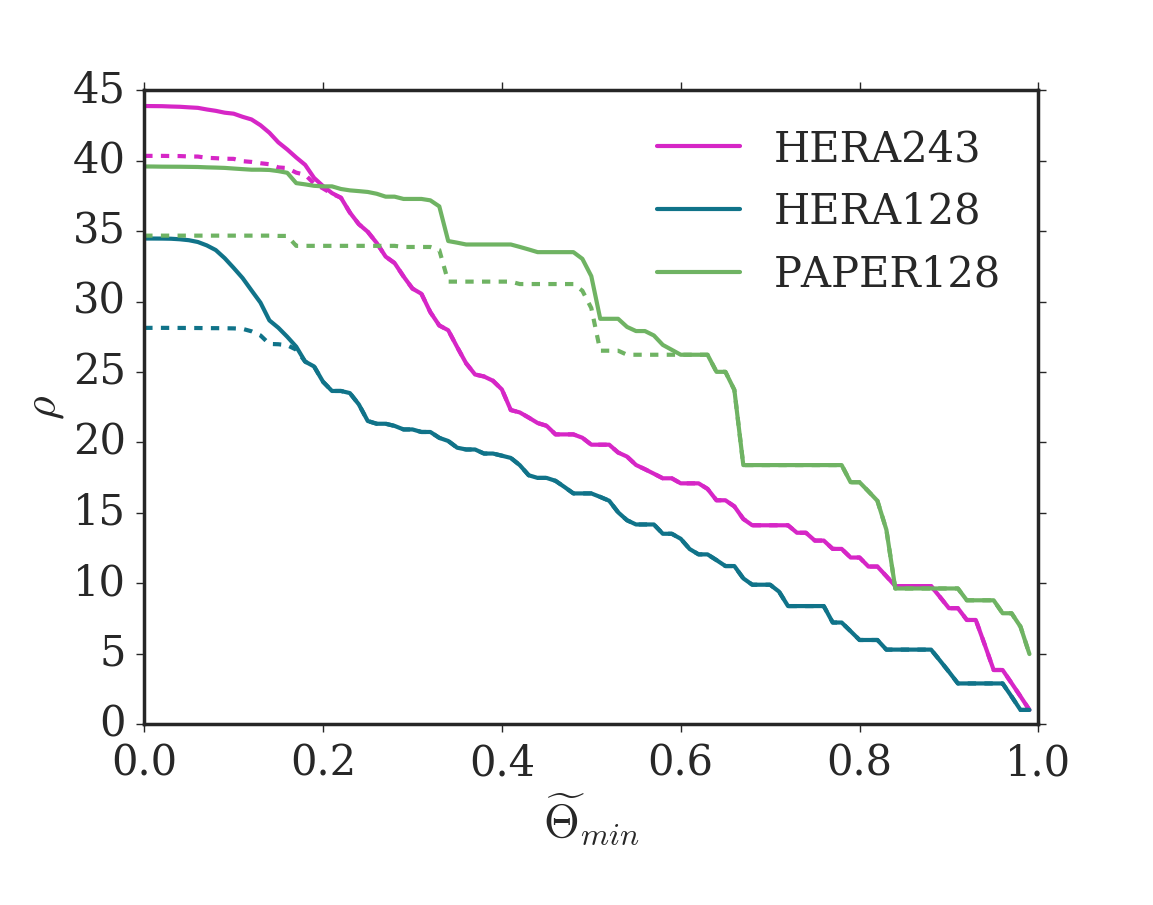
\includegraphics[width=\linewidth]{osens}
\caption{Sensitivity of redundant arrays as a function of the minimum effective weight. Dashed lines represent when only equivalent baseline pairs are used, while solid lines indicate use of both the equivalent and near-equivalent baselines are used. The y-axis is normalized independently for each array such that the contribution of the top single equivalent pair class is unity, and thus does not indicate a comparison of absolute sensitivity across the different arrays shown.  }
\label{fig:osens}
\end{figure}
%\end{centered}











%\subsection{Notes on Data, Foreground and Noise}
%Unlike the simulated clean EOR signal, real data are dominated by foreground %and thermal noise, neither of which turns out to exhibit the correlation %pattern seen in Fig.  \ref{fig:numerics}. Foreground exhibits long-range %correlations and would lead to high responses at wide range of time-offsets. %Instrumental noise for different baselines/antenna-pairs, on the other hand, are uncorrelated and thus exhibit responses consistent with zero at all time offsets. 
%To illustrate, we use the second observing season of PAPER-128 data, taken from Jan. 21st to March 7th of 2014. To illustrate the effect of noise and foreground, we use the data before fringe-rate and delay filtering. 

\section{Conclusion}
Redundant arrays are designed to maximize sensitivity. Current generations of redundant radio arrays, such as those probing the power spectrum of the epoch of reionization could benefit from data analysis techniques that improve the sensitivity. We present an intuitive analysis of cross-multiplying baselines that are close in length and orientation to each other. Given an antenna array configuration, our method quickly identifies the best baseline pairs to cross-multiply and predict the expected sensitivity contribution. With the predicted result one can improve existing power-spectrum pipelines through 3 simple steps. 1). Rephase the visibilities prior to delay transforming by the zenith displacement (or more accurately by the phase predicted by our numerical analysis). 2). Shift the visibilities in time. 3) Cross multiply the visibilities of the two baselines  to form the power spectrum. 4) Finally combine the different baseline pairs by appropriate inverse-variance weighting that takes into account the predicted sensitivity contributions of each case. We showed that such techniques could lead to $20\%$ to $60\%$ increase in sensitivity for PAPER and HERA. 


\pagebreak



\appendix
\section{\label{sec:appB}\\Derivation of Noise Covariance \label{sec:appB}}
\label{sec:appB}
In this appendix we give a brief derivation of the effective weight quoted in \ref{sec:sensitivity}. We combine the different power spectrum measurements by inverse variance weighting \footnote{In practice techniques such as bootstrapping is often used, see for example \citep{Ali2015}}. We shall separate the visibility and power spectrum into signal and noise contributions:
\begin{equation}
\begin{aligned}
V &= V_S+V_N,\\
P &= P_S+P_N.
\end{aligned}
\end{equation}
We shall denote the noise variance of power spectrum and visibility
\begin{equation}
\begin{aligned}
\sigma_V^2 &= \langle |V_N|^2 \rangle,\\
\sigma_P^2 &= \langle P_N^2 \rangle.
\end{aligned}
\end{equation}
One may notice that we have used a single covariance for the complex quantity visibility. It's simple to show that the same result holds if we use a separate real and imaginary components, as long as they are independent of each other. In fact, for simplicity and without loss of generality we shall treat the visibility as a real quantity in the rest of this derivation. 
Note that though we can assume $\langle V_N^{odd-power}\rangle=0$, the same is not true for $P_N$. 

Then the variance of $P$ constructed with visibilities $V_1$ and $V_2$ from two baseline classes can be estimated\footnote{We assume all noise terms to be independent for simplicity, in practice the correlation of different measurements ifrom equivalent baselines are alleviated by grouping the baselines in the class and the days of observation, as in \cite{Ali2015}}:
\begin{equation}
\begin{aligned}
\sigma_P^2 &= \langle P^2\rangle -\langle P \rangle^2,\\
&\propto \langle \frac{(V_{1S}+V_{1N})^2 (V_{2S}+V_{2N})^2}{\Theta^2} \rangle - \langle \frac{(V_{1S}+V_{1N}) (V_{2S}+V_{2N})}{\Theta} \rangle ^2,\\
&= \frac{1}{\Theta^2} \left( V_{1S}^2\sigma_{V2}^2+V_{2S}^2\sigma_{V1}^2+\langle V_{1N}^2 V_{2N}^2\rangle\right), \\
&= \frac{1}{\Theta^2} \left[ V_{S}^2(\sigma_{V2}^2+\sigma_{V1}^2) + \sigma_{V1}^2 \sigma_{V2}^2\right], 
\end{aligned}
\end{equation}

where in the second last line we have substituted visibility noise variance. In the final line we used Wick's theorem and the fact that the signal from two visibilities are equal. 

Recall from the discussion on multiplicities we can write
\begin{equation}
\sigma_V^2=\frac{\sigma_0^2}{M},
\end{equation}
where $\sigma_0$ is some single-baseline noise level. Letting $\rho_0=V_S^2/\sigma_0^2$ be the signal to noise ratio for a single baseline, we can write

\begin{equation}
\begin{aligned}
\sigma_P^2 & \propto  \frac{\sigma_0^4}{\Theta^2} \left[ \rho_0 \left(\frac{1}{M_1}+\frac{1}{M_2} \right) + \frac{1}{M_1 M_2}\right], \\
&\propto \frac{1}{\widetilde{\Theta}_{12}^2},
\end{aligned}
\end{equation}
where we have defined a slightly modified version of the effective weight (compare with Eq. \ref{eq:sensul}):
\begin{equation}
\widetilde{\Theta}_{12}=\frac{\Theta_{12}\sqrt{M_1M_{2}}}{\sqrt{1 + \rho_0 \left(M_1+M_{2} \right)}}.
\end{equation}







\bibliographystyle{apj}
%\nocite{*}
\bibliography{draft_working}

\end{document}
